\chapter{Evaluation}
The system presented exploits non-volatile memory to save data to be retained in the event of a power failure. The novelty of this implementation is the resistance to data loss in case of power failure added to the implementation of the TRAP protocol to reduce this type of events. To better highlight this progress, this chapter mainly presents some emulations performed with the presented stack, compared with emulations without the provided implementation.
\label{cha:Evaluation}
%memory overhead of implementation
\section{Technical details}
\label{sec:Technical deatils}
The size of the implementation varies according to the number of nodes within the network, the size of the RX and TX buffers saved in FRAM, and the optimization required of the compiler. 
For compiling optimization the highest level (Whole Program Optimization) is used, this also helps to reduce the power consumption of the system \cite{OptimizationCompiler}.\\
To provide some data, with 2 nodes in the network and the receive and send buffer (buffer RX and buffer TX) of size 3, the memory overhead is 5223 bytes.\\
The figure below shows the memory allocation provided by the Code Composer Studio IDE.\\
\begin{figure}[H]
\centerline{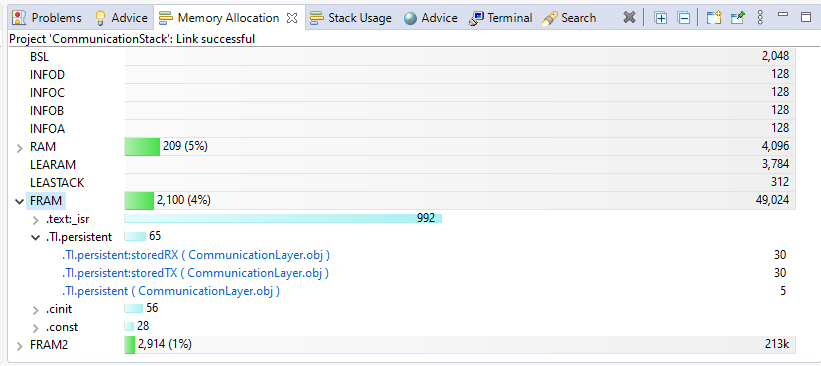
\psfig{file=Images/memoryOverhead.png,width=0.7\textwidth}}
\caption{\footnotesize \centering Memory overhead for network with 2 nodes and buffer size 3}
\label{fig:memoryOverhead}
\end{figure}
If the network nodes are increased to 16 and the size of both buffers to 32, the overhead will be 5307 bytes.\\
It is then possible to estimate the memory overhead of the implementation at about 5.5KB.
\section{Emulation}
\label{sec:Simulation}
The setup used for the emulations involves communication between two nodes; consequently, two TI MSP430 boards were used:
\begin{enumerate}
\item TI MSP430FR5994
\item TI MSP430FR5969
\end{enumerate}
For communication regarding the energy level (TRAP Layer), the backscatter channel was emulated using a wired connection. However, the operation is similar to using RF for transmission; in fact, it is based on toggling a GPIO pin for sending and generating external GPIO interrupts for receiving.\\
Communication between nodes for sending data is via the UART and is therefore also wired.\\
The choice to use UART rather than a GPIO pin to send the packet bit by bit was dictated by the difficulty of managing the latter implementation. Using a GPIO pin and sending either a high value or a low value depending on the bit value of the sequence to be sent would require sampling the signal at the sending frequency. This would result in adding complexity to the system.\\
In any case, since the communication stack presented is modular, replacement of the Physical Layer from UART to an implementation working with other types of communications does not require modification of the upper layers.\\
To observe the behavior of the nodes, a wired connection was made between the computer and the boards through another UART.\\\\
Tests consist of 20 minutes of emulated system operation;
it is important to note that these tests are limited to a short period of time and to limited cases. In order to get a more realistic overview of system performance, longer tests need to be conducted.\\
\begin{figure}[H]
\centerline{\psfig{file=Images/testBed.jpg,width=0.7\textwidth}}
\caption{\footnotesize \centering Test bed with MSP430FR5994 on the left and MSP430FR5969 on the right, white wires are for TRAP Layer, red wires are for data transmission}
\label{fig:testBed}
\end{figure}
\subsection{Energy Params For Emulation}
During the emulations, we do not have a system that can collect energy from its surroundings; therefore, the node capacitor is charged by a power source based on a random generation function.\\
The average percent increase in capacitor charge per second is declared before the test results.\\
Capacitor energy is consumed for data collection from the environment and forwarding to the application layer; this consumption during the emulation is fixed at 32\% of the maximum capacity.\\
Data transmission requires, in this emulation, a charge level of 64\% or more of the maximum capacitance of the capacitor, unlike reception, for which consumption of 62\% of the capacitance of the capacitor is simulated.\\
These estimated consumption values were decided by taking as reference a 2mF capacitor, a BGM220S BLE module \cite{BLEModule} for transmission, and a DHT11 humidity and temperature sensor \cite{DHT11Module} to collect the data from the surrounding environment.\\
Compared to SRAM, FRAM access results in a somewhat higher power consumption \cite{MSP430FRAMDS}, so when the stack is used, an additional 1\% consumption will be added to these values. In fact, the FRAM is used in receiving to save the data, in sending to retrieve the data, and in producing the packet to do the saving.\\
It is important to point out that the values presented are used only for emulation and do not reflect exactly the real capacitor capacity and consumption of the board.\\
When the simulated charge level of the capacitor reaches 0\%, the node is reset. To reset the node, an instruction from an invalid memory allocation is fetched.\\
Energy status update period is set to 1. This data item indicates every when the node energy information is sent to the network.
\subsection{Production Of Packages During The Emulation}
Data production on the nodes was simulated at fixed intervals, the emulations were performed with two different production patterns.\\
For the first test group, data was produced repeatedly every 60 seconds on the first node and every 90 seconds on the second node.\\
For the second test group, data was produced repeatedly every 60 seconds on the first node and every 75 seconds on the second.\\
This is useful for understanding the performance of the system with different production patterns.
\subsection{First test group}
\label{sec:FT}
In this first set of emulations, the operation of the system with and without the presented stack is tested. The energy level of the nodes is sent via Layer TRAP, and packets are produced repeatedly every 60 seconds on one node and every 90 seconds on the other.\\
Summary of the parameters of the emulation group:\\\\
\begin{tabular}{lll} \hline
Packet production repetition time on node 1: & 60 seconds\\ \hline
Packet production repetition time on node 2: & 90 seconds\\ \hline
Energy status update period: & 1 second \\ \hline
Simulated energy consumption in TX: & 64\% (+1\% if the stack is used) \\ \hline
Simulated energy consumption in RX: & 62\% (+1\% if the stack is used)\\ \hline
Simulated energy consumption for packet production: & 32\% (+1\% if the stack is used)\\ \hline
\end{tabular}
\begin{enumerate}
\item First emulation: average energy increment 0.71\% per second\\
For the first test an average energy growth per second inside the capacitor of about 0.71\% is emulated.\\
The result with the stack presented shows the sending of 5 packets and the successful reception of 5 packets, as opposed to not using it with which a result of 8 packets sent and 0 packets received is obtained (Figure \ref{fig:FGFT0}).\\
The success rate is then 100\% using the stack and 0\% without using the presented implementation.\\
It is important to note that fewer packets are sent with the use of the stack than with emulation without the stack. This result is closely related to the delay introduced by the TRAP protocol to allow the nodes to reach the correct energy level before starting transmission.\\
However, it is certainly better to successfully transmit fewer packets than to send more packets but not be sure of correct reception by the receiving node.
\begin{figure}[H]
\centerline{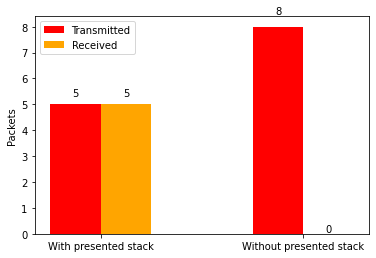
\psfig{file=Images/9060071MatPlot.png,width=0.5\textwidth}}\caption{\footnotesize \centering Emulation results with average energy increment of 0.71\% per second}
\label{fig:FGFT0}
\end{figure}
\begin{comment}
\begin{figure}[H]
\centerline{\psfig{file=Images/9060071RATIO.png,width=0.7\textwidth}}
\caption{\footnotesize \centering Success ratio of transmission with average energy increment of 0.71\% per second}
\label{fig:FGFT1}
\end{figure}
\end{comment}
\item Second emulation: average energy increment 1.25\% per second\\
This second emulation assumes an average energy growth of 1.25\% of the capacitor capacity per second.\\
If we go to analyze the data obtained from the tests, we can see that the results without using the stack are slightly better than what was seen in the previous emulations. This improvement is due to higher average energy growth.\\
In any case, the results obtained with the stack presented are still better than those obtained without using any protocol.
\begin{figure}[H]
\centerline{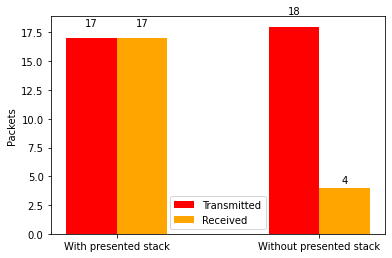
\psfig{file=Images/9060125MatPlot.png,width=0.5\textwidth}}
\caption{\footnotesize \centering Emulation results with average energy increment of 1.25\% per second}
\label{fig:FGST0}
\end{figure}
\begin{comment}
\begin{figure}[H]
\centerline{\psfig{file=Images/9060125RATIO.png,width=0.7\textwidth}}
\caption{\footnotesize \centering Success ratio of transmission with average energy increment of 1.25\% per second}
\label{fig:FGST1}
\end{figure}
\end{comment}
\item Third emulation: average energy increment 2\% per second\\
Following the trend of previous tests, the average value of per-second increment of energy within the capacitor is also changed in these emulations. In particular, an average increment of 2\% is proposed.\\
Similar to what highlighted in the previous test, the result without the stack achieves a higher transmission success rate than the first case presented, this increase is due to a higher growth of the energy inside the capacitor.\\
However, the stack allows the system to achieve better performance.\\
It is interesting to note that, during this emulation, the number of total transmissions using the stack is higher than the number of transmissions without the stack (Figure \ref{fig:FGTT0}). This increase in transmissions is due to the saving of packets already produced in non-volatile memory and consequently as soon as possible the saved packets are sent without waiting for a new production.
\begin{figure}[H]
\centerline{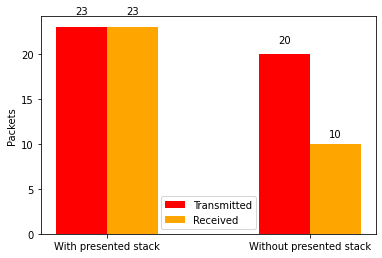
\psfig{file=Images/90602MatPlot.png,width=0.5\textwidth}}
\caption{\footnotesize \centering Emulation results with average energy increment of 2\% per second}
\label{fig:FGTT0}
\end{figure}
\begin{comment}
\begin{figure}[H]
\centerline{\psfig{file=Images/90602RATIO.png,width=0.7\textwidth}}
\caption{\footnotesize \centering Success ratio of transmission with average energy increment of 2\% per second}
\label{fig:FGTT1}
\end{figure}
\end{comment}
\end{enumerate}
\newpage
\subsection{Second test group}
\label{sec:ST}
This second group of emulations follows the same energy pattern presented with the previous group; however, having different periods for packet production the results obtained in relation to the number of transmissions are slightly different. The production periods are set to 60 seconds for the first node and 75 seconds for the second.\\
Summary of the parameters of the emulation group:\\\\
\begin{tabular}{lll} \hline
Packet production repetition time on node 1: & 60 seconds\\ \hline
Packet production repetition time on node 2: & 75 seconds\\ \hline
Energy status update period: & 1 second \\ \hline
Simulated energy consumption in TX: & 64\% (+1\% if the stack is used)\\ \hline
Simulated energy consumption in RX: & 62\% (+1\% if the stack is used)\\ \hline
Simulated energy consumption for packet production: & 32\% (+1\% if the stack is used)\\ \hline
\end{tabular}
\begin{enumerate}
\item First emulation: average energy increment 0.71\% per second\\
The first emulation assumes a percentage energy growth of 0.71\% of the capacitor capacity per second.\\
It can be seen from the results obtained that the number of successful transmissions is significantly higher if the presented stack is used (Figure \ref{fig:SGFT0}).\\
The result is particularly significant in that it shows that, in the case of low energy growth within the node, the presented stack, due to the implementation of the TRAP protocol, performs better than not using any control during transmission.\\
Again, the lower number of transmission actions observable with the use of the stack is due to the TRAP protocol delaying sending until the energy levels required to successfully complete the transmission are reached.
\begin{figure}[H]
\centerline{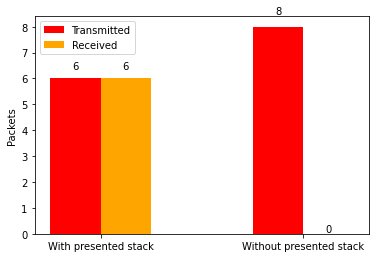
\psfig{file=Images/7560071MatPlot.png,width=0.5\textwidth}}
\caption{\footnotesize \centering Emulation results with average energy increment of 0.71\% per second}
\label{fig:SGFT0}
\end{figure}
\begin{comment}
\begin{figure}[H]
\centerline{\psfig{file=Images/7560071RATIO.png,width=0.7\textwidth}}
\caption{\footnotesize \centering Success ratio of transmission with average energy increment of 0.71\% per second}
\label{fig:SGFT1}
\end{figure}
\end{comment}
\item Second emulation: average energy increment 1.25\% per second\\
Also in this tests, results obtained with the stack are better in relation to the one without.\\
However, it is interesting to note that, with a higher energy growth than in the previous test, more packets can be sent using the stack. This increase is due to the use of FRAM memory by the stack, which then creates a persistent queue of packets to be sent that is not dropped on power failure.
\begin{figure}[H]
\centerline{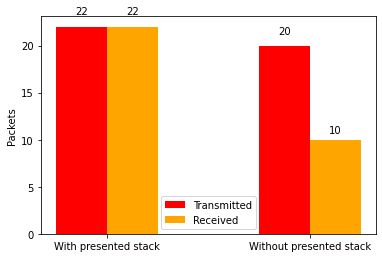
\psfig{file=Images/7560125MatPlot.png,width=0.5\textwidth}}
\caption{\footnotesize \centering Emulation results with average energy increment of 1.25\% per second}
\label{fig:SGST0}
\end{figure}
\begin{comment}
\begin{figure}[H]
\centerline{\psfig{file=Images/7560125RATIO.png,width=0.7\textwidth}}
\caption{\footnotesize \centering Success ratio of transmission with average energy increment of 1.25\% per second}
\label{fig:SGST1}
\end{figure}
\end{comment}
\item Third emulation: average energy increment 2\% per second\\
The third test presents very similar results (Figure \ref{fig:SGTT0}) to those described in the second test (Figure \ref{fig:SGST0}), also in this emulation the success ratio of the stack is 100\% as opposed to the one without the stack which is significantly lower (about 37\%).\\
We can also highlight in this test the higher number of packets sent using the stack despite the delay in transmission introduced by the TRAP protocol to achieve the energy levels required for successful transmission.
\begin{figure}[H]
\centerline{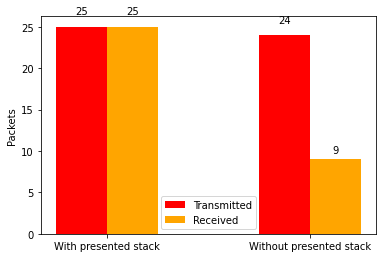
\psfig{file=Images/75602MatPlot.png,width=0.5\textwidth}}
\caption{\footnotesize \centering Emulation results with average energy increment of 2\% per second}
\label{fig:SGTT0}
\end{figure}
\begin{comment}
\begin{figure}[H]
\centerline{\psfig{file=Images/7560125RATIO.png,width=0.7\textwidth}}
\caption{\footnotesize \centering Success ratio of transmission with average energy increment of 2\% per second}
\label{fig:SGTT1}
\end{figure}
\end{comment}
\end{enumerate}
\section{Results Discussion}
\label{sec:SimulationDiscussion}
The tests carried out showed that in the case of using the stack presented in this thesis, the performance of the system in terms of successfully sent packets goes up significantly.\\
Calculating an average relative to the success rate obtained with the stack we observe that is almost 70 percentage points higher than the result obtained without the use of any protocol (Figures \ref{fig:FTA}).

\begin{figure}[H]
\centerline{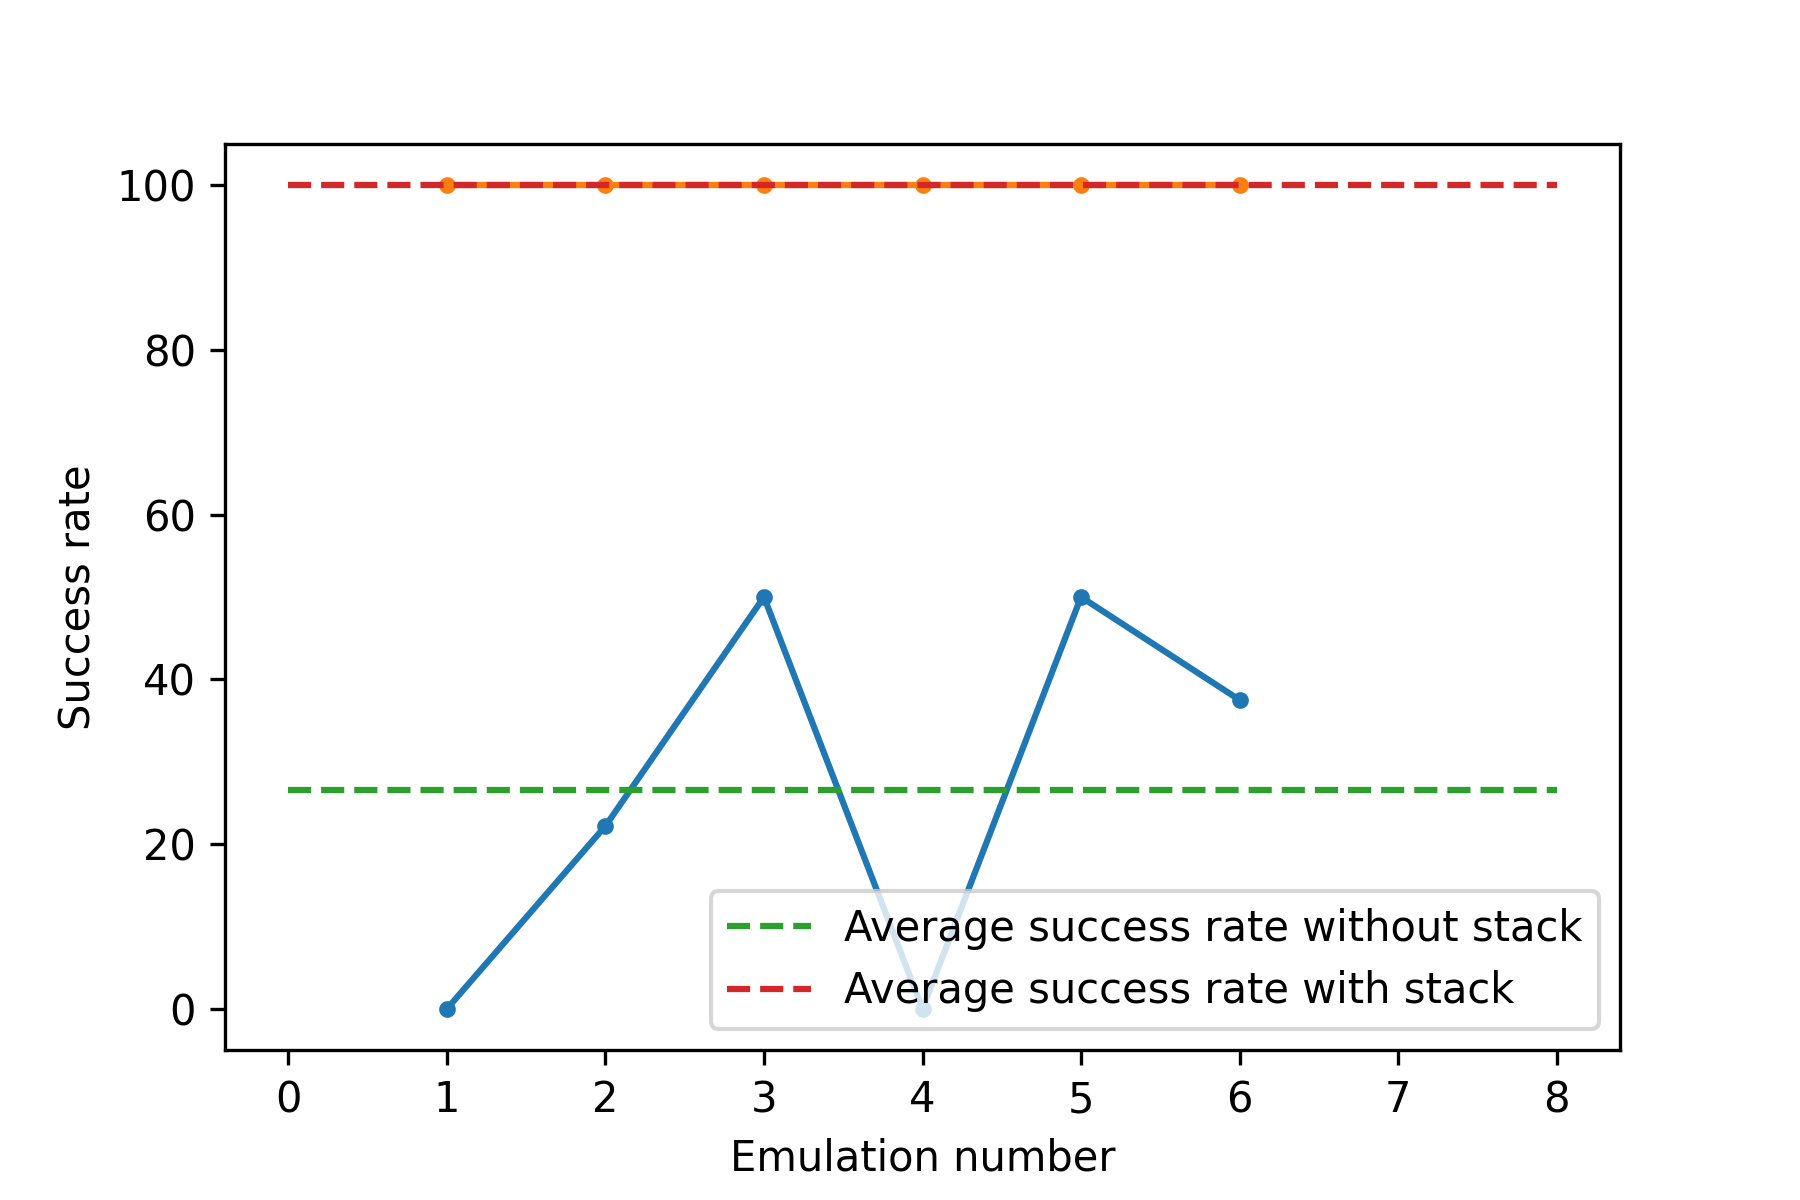
\psfig{file=Images/finalAverage.png,width=0.7\textwidth}}
\caption{\footnotesize \centering Plot representing the success rate in transmission obtained with and without the presented stack. The dashed line represents the average value obtained. The stack improves system performance by almost 70\%.}
\label{fig:FTA}
\end{figure}

In particular, it can be seen that under conditions in which the capacitor is charged by an energy source capable of providing only a small percentage charge per second (Figure \ref{fig:FGFT0} and Figure \ref{fig:SGFT0}) the performance of the system using the presented stack is very good in relation to the number of packets successfully sent.\\
This improvement is mainly due to the use of the TRAP protocol to make the node aware of the energy level of neighboring nodes and thus avoid wasting energy on transmissions that cannot be completed.\\\\
It is important to remember how the tests were not run for long periods of time and how they did not take into account all possible situations that the system might encounter during ordinary operation. However, they do allow for a general idea regarding the performance of the system with and without the use of the presented stack.
\newpage




